\section{Zadanie 1}
\autor{Mateusz Wojaczek}
Wiewiórka chodzi po skończonej kracie jak na rysunku poniżej w sposób losowy. 
Rozpoczyna swoją trasę w wierzchołku $(0,0)$ i w każdym kroku wybiera w sposób losowy, jednostajny i niezależny jeden z sąsiednich wierzchołków aktualnego wierzchołka.
W wierzchołku $(1,1)$ znajduje się żołądź. 
Należy wyznaczyć oczekiwaną liczbę kroków potrzebnych, aby wiewiórka dotarła do żołędzia.


\subsection*{Rozwiązanie}
Ze względu na symetrię wystarczy rozważyć połowę kwadratu:


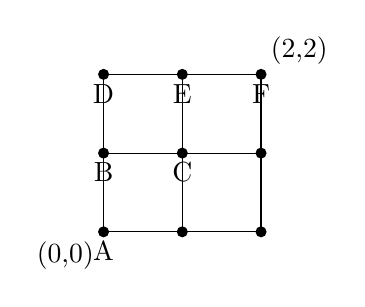
\begin{tikzpicture}
    \coordinate (A) at (0,0);
    \coordinate (B) at (1,0);
    \coordinate (C) at (2,0);
    \coordinate (D) at (0,1); 
    \coordinate (E) at (1,1);
    \coordinate (F) at (2,1);
    \coordinate (G) at (0,2);
    \coordinate (H) at (1,2);
    \coordinate (I) at (2,2);

    

    % Draw the grid
    \draw (A) grid (I);

    % Draw dots at each coordinate
    \foreach \point in {A,B,C,D,E,F,G,H,I} {
        \fill (\point) circle (2pt);
    }

    % Label the corners (0,0) and (1,1) as in the original image
    \node[below left] at (A) {(0,0)};
    \node[above right] at (I) {(2,2)}; % Adjusted to (2,2) for the 3x3 grid

   

    \node[below] at (A) {A}; % (0,0)
    \node[below] at (D) {B}; % (0,1)
    \node[below] at (E) {C}; % (1,1)
    \node[below] at (G) {D}; % (0,2)
    \node[below] at (H) {E}; % (0,2)
    \node[below] at (I) {F}; % (0,2)
\end{tikzpicture}

\section*{Rozwiązanie}

Oznaczmy oczekiwane liczby kroków z poszczególnych wierzchołków odpowiednio:
\[
A = E(0,0), \quad
B = E(1,0), \quad
C = E(1,1), \quad
D = E(2,0), \quad
E = E(2,1), \quad
F = E(2,2)
\]
Ponieważ wierzchołek $(2,2)$ zawiera żołądź, mamy
\[
F = 0.
\]

Dla pozostałych wierzchołków zapisujemy równania dla wartości oczekiwanej:

\[
\begin{cases}
A = 1 + B, \\[6pt]
B = 1 + \frac{1}{3}A + \frac{1}{3}C + \frac{1}{3}D, \\[6pt]
C = 1 + \frac{1}{2}B + \frac{1}{2}E, \\[6pt]
D = 1 + \frac{1}{2}B + \frac{1}{2}C, \\[6pt]
E = 1 + \frac{1}{3}C + \frac{1}{3}D + \frac{1}{3}F.
\end{cases}
\]

Ponieważ $D = C$ , układ upraszcza się do:

\[
\begin{cases}
A = 1 + B, \\[6pt]
B = 1 + \frac{1}{3}A + \frac{2}{3}C, \\[6pt]
C = 1 + \frac{1}{2}B + \frac{1}{2}E, \\[6pt]
E = 1 + \frac{2}{3}C.
\end{cases}
\]

Z ostatniego równania otrzymujemy:
\[
E = 1 + \frac{2}{3}C.
\]

Podstawiając do trzeciego równania:
\[
C = 1 + \frac{1}{2}B + \frac{1}{2}\left(1 + \frac{2}{3}C\right),
\]
czyli
\[
C = \frac{3}{2} + \frac{1}{2}B + \frac{1}{3}C.
\]
Stąd
\[
\frac{2}{3}C = \frac{3}{2} + \frac{1}{2}B \quad \Rightarrow \quad C = \frac{9}{4} + \frac{3}{4}B.
\]

Podstawiając do równania dla $B$:
\[
B = 1 + \frac{1}{3}A + \frac{2}{3}C.
\]
Z $A = 1 + B$ mamy:
\[
B = 1 + \frac{1}{3}(1 + B) + \frac{2}{3}C,
\]
czyli
\[
\frac{2}{3}B = \frac{4}{3} + \frac{2}{3}C \quad \Rightarrow \quad B = 2 + C.
\]

Podstawiamy $C = \frac{9}{4} + \frac{3}{4}B$:
\[
B = 2 + \frac{9}{4} + \frac{3}{4}B,
\]
czyli
\[
\frac{1}{4}B = \frac{17}{4} \quad \Rightarrow \quad B = 17.
\]

Stąd:
\[
C = \frac{9}{4} + \frac{3}{4} \cdot 17 = \frac{9 + 51}{4} = 15, \quad A = 1 + B = 18.
\]

Oczekiwana liczba kroków, jakie wiewiórka wykona zanim znajdzie żołędzia, wynosi \(\mathbf{18}\).

\subsection*{Odpowiedź}
\[
\boxed{\text{18}}
\]
